\documentclass[tikz,border=2pt]{standalone}
\usepackage[T1]{fontenc}
\usepackage[utf8]{inputenc}
\usepackage{lmodern}
\usepackage{pgfplots}
\pgfplotsset{compat=1.17}
\begin{document}
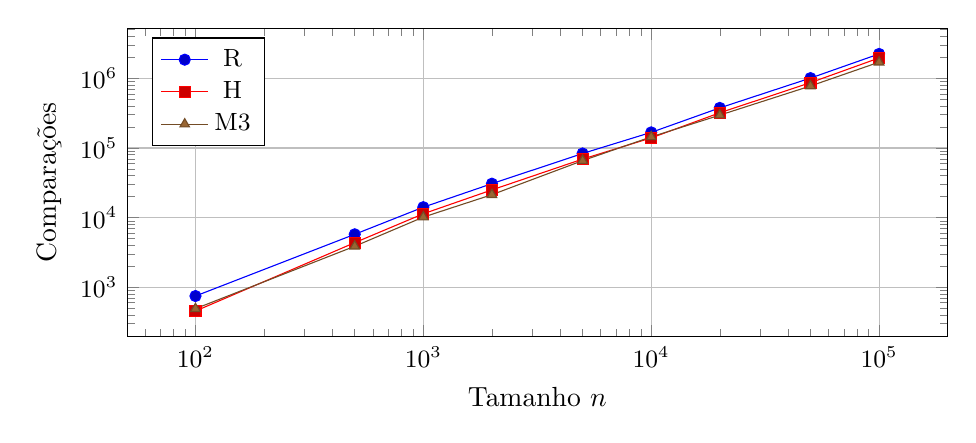
\begin{tikzpicture}
\begin{axis}[width=12cm,height=5.5cm,xmode=log,ymode=log,xlabel={Tamanho $n$},ylabel={Comparações},grid=major,legend pos=north west,legend style={font=\small},tick label style={font=\small}]
\addplot+[mark=*] coordinates {(100,749) (500,5768) (1000,14135) (2000,30732) (5000,83425) (10000,167611) (20000,376521) (50000,1008325) (100000,2240874)};
\addlegendentry{R}
\addplot+[mark=square*] coordinates {(100,456) (500,4372) (1000,11363) (2000,25016) (5000,69296) (10000,139666) (20000,320318) (50000,867115) (100000,1960416)};
\addlegendentry{H}
\addplot+[mark=triangle*] coordinates {(100,493) (500,3883) (1000,10182) (2000,21355) (5000,65824) (10000,144327) (20000,296273) (50000,776512) (100000,1706146)};
\addlegendentry{M3}
\end{axis}
\end{tikzpicture}
\end{document}
